\documentclass[a4paper,11pt]{book}

%\usepackage{xspace}
\usepackage[T1]{fontenc}
%\usepackage{palatino}
% \usepackage[dvips,dvipdf]{graphics}
\usepackage{graphics}
\usepackage{epsfig}
\usepackage{url}
\usepackage{a4wide}
%\usepackage{boxedminipage}
%\usepackage{calc}
\usepackage{fancybox}
\usepackage{alltt}
%\usepackage{moreverb}
\usepackage{longtable}
\usepackage{array}
\usepackage[dvipsnames,usenames]{color}
\usepackage{xcolor}
\usepackage{makeidx}
%\usepackage{rotating}
%\usepackage{sectionbox}
\usepackage{listings}

\definecolor{RED}{rgb}{1,0,0}

\lstdefinestyle{C++}{
  language=C++, % the language of the code
  basicstyle=\scriptsize, % the size of the fonts that are used for the code
  basicstyle=\ttfamily, % Without beramono, we'd get cmtt, the teletype font.
  % commentstyle=\textit, % cmtt doesn't do italics. It might do slanted text though.
  commentstyle=\color{Emerald}\itshape,
  keywordstyle=\color{DarkOrchid}\bfseries,
  % fontadjust,
  % numbers=left, % where to put the line-numbers
  % numberstyle=\tiny, % the size of the fonts that are used for the line-numbers
  % stepnumber=2, % the step between two  line-numbers.  If it's 1, each line will
		% be numbered
  % numbersep=5pt, % how far the line-numbers are from the code
  % showspaces=false, % show spaces adding particular underscores
  showstringspaces=false, % underline spaces within strings
  % showtabs=false, % show tabs within strings adding particular underscores
  % frame=llines, % adds a frame around the code
  % frame=tb,
  tabsize=2, % sets default tabsize to 2 spaces
  captionpos=b, % sets the caption-position to bottom
  breaklines=true, % sets automatic line breaking
  breakatwhitespace=false,   % sets if  automatic breaks  should only  happen at
			    % whitespace
  % title=\lstname, % show the filename of files included with \lstinputlisting;
  % also try caption instead of title
  % escapeinside={\%*}{*)}, % if you want to add a comment within your code
  xleftmargin=1cm,
  xrightmargin=1cm,
  mathescape=true,
  escapechar=\%,
  morekeywords={Real, UInt, Int},
  columns=flexible,
  keepspaces=true,
  backgroundcolor=\color{GreenYellow}
}

\lstnewenvironment{cpp}{\lstset{style=C++}}{}

\makeatletter
\def\lst@outputspace{{\ifx\lst@bkgcolor\empty\color{white}\else\lst@bkgcolor\fi\lst@visiblespace}}
\makeatother


\lstnewenvironment{command}{\lstset{
    language=bash,
    backgroundcolor=\color{Salmon},
    breaklines=true}}{}


\usepackage[pdftex,
            hyperindex=true,
            pagebackref=true,
            colorlinks=true,
            linkcolor=blue,
            anchorcolor=magenta,
            citecolor=blue,
            urlcolor=blue,
            unicode,
            implicit=true
            ]{hyperref}

% \usepackage{ae}
% \usepackage{aecompl}
% \usepackage[cm]{aeguill}
% \usepackage{times}
% \usepackage{bookman}
\usepackage{palatino}
\usepackage{verbatim}
\usepackage{xspace}

\sloppy
\newcommand{\version}{0.1}

\newcommand{\akantu}{\texttt{\textbf{Akantu}}\xspace}
\newcommand{\code}[1]{\texttt{#1}}
\newcommand{\note}[1]{\textbf{Note: }\textit{#1}}
\newcommand{\todo}[1]{~({\small\color{red}\textbf{TODO: }\textbf{#1}})}




\bibliographystyle{plain}

\title{\textbf{\Huge AKANTU}\\
  \vspace{0.5cm}
  \textbf{\huge User's Guide}\\
  \vspace{1cm}
  {\small \today{} --- Version \version}
}

\date{}

\makeindex

\begin{document}

\maketitle

\tableofcontents

\chapter{Introduction}

% \section{Data structures\label{chap:data-structure}}

% \subsection{Vectors\label{sec:vectors}}

% The Vector class is a template class  that can store scalar types as Real, UInt,
% Int  or bool.   A Vector  instance is  defined  by its  size and  its number  of
% component.  It also  has an  identifier and  some extra  internal  variables for
% memory handling purpose.

% \begin{itemize}
% \item The size is the number of tupels stored in the Vector.
% \item The number of component is the number of values stored for each tuple.
% \end{itemize}

% \begin{figure}[!htb]
%   \centering
%   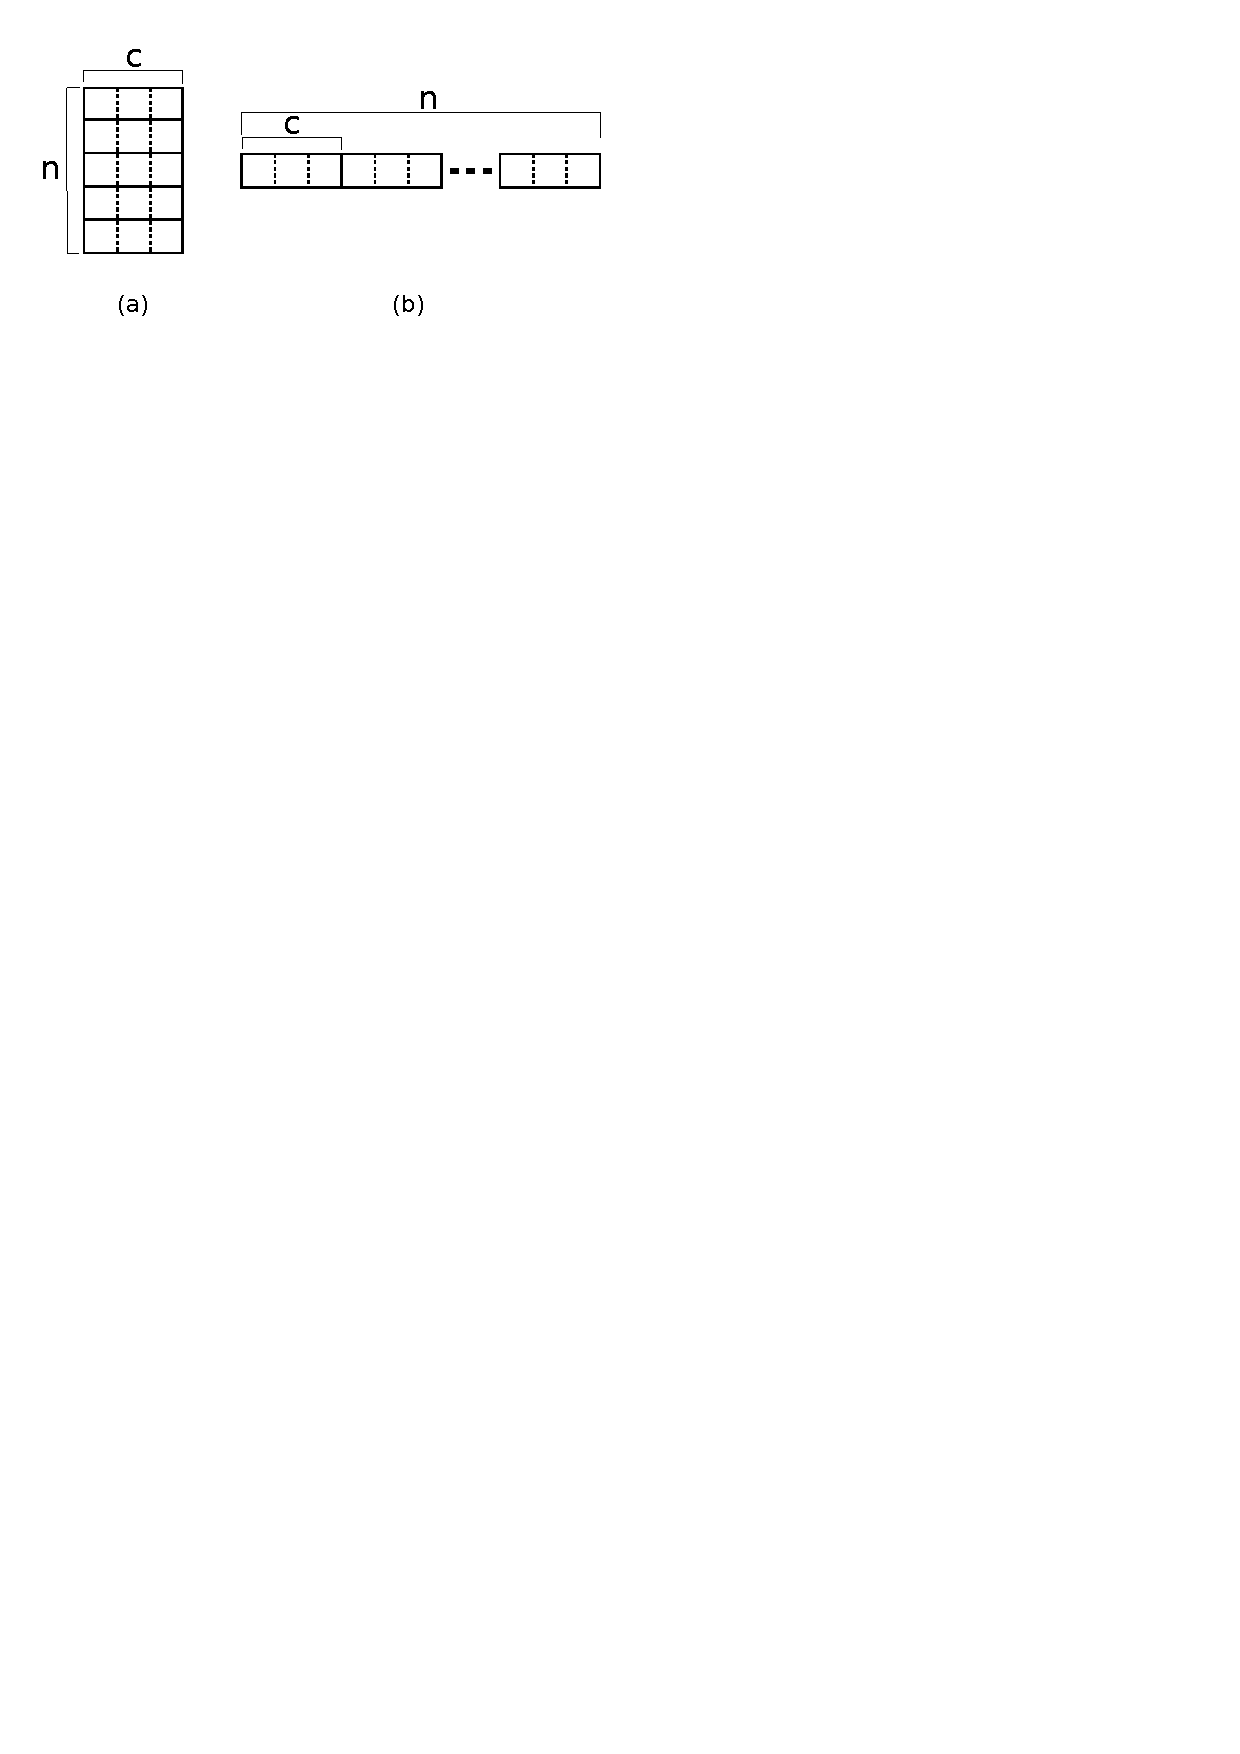
\includegraphics{figures/vectors}
%   \caption{View of  a Vector of size  n and c compenents,  (a) representation of
%     the vector, (b) representation of the storage of the same Vector.}
%   \label{fig:vectors}
% \end{figure}

% All the  data are linerarized  in memory in  an array called values.  This class
% member is public.  So for a Vector  of size $n$ and $c$ component, to access the
% $j^{th}$  component of  th  $i^{th}$ tuple,  you have  to  get $values[i  * c  +
% j]$. You  can also  access to this  value with  accessor \code{at(i, j)}  or the
% constant accessor \code{get(i, j)}.

% If  you want to  store a  matrix on  each tuple  you have  to linearize  it. For
% exemple if you want to store a m * k matrix on each tuple you must specify c = m
% * k.  To access a particular value  in a matrix of  a tuple you will  have to do
% something like $values[ i * m * k + j_i * m + j_j]$.

% \subsubsection{Vector storage convention within FE object\label{sec:FE-convention}}

% The point of  this section is to describe the convention  of storage for vectors
% intented  to be  passed to  {\bf  FE} object  methods.  Indeed  a convention  of
% necessary  since gradient  operators or  integrtaion loops  will use  vectors as
% input and ouput.   Such vectors will be ordered with  a specific convention that
% we intend to describe now.

% For  vector objects,  the  size of  the vector  is  always the  number of  nodes
% associated.  The number  of components  is related  to the  order of  the tensor
% considered. For a scalar  field it is 1, for a vectorial  field, the size of the
% vector is the number of components. For a $m\times n$ matrix field the number of
% components is $m\times n$.

% One common operation  is the manipulation of continuum  fields at the quadrature
% point  positions.   Here  the  size   of  the  vector  is   $mn\_element  \times
% nb\_quad\_points$  and  the  number  of  components is  related  to  the  stored
% object.  For instance the  method \verb$interpolateOnQuadraturePoints()$  take a
% nodal field  stored in a  vector($n\_nodes$,$dim$) and return  a vector($n\_elem
% \times n\_quads$,$dim$).

% Basic gradient operations, like method \verb$gradientOnQuadraturePoints()$, will
% take  as input a  vector($n\_nodes$,$dim$) and  return a  vector($n\_elem \times
% n\_quads$,$dim \times spatial\_dimension$) where spatial dimension is the number
% of dimension in which the domain is embedded.

% In  the  same  way   the  integration  routines  expect  vector($n\_elem  \times
% n\_quads$,$dim$)  and  will  return vector($n\_elem$,$dim$).   For  non-Gaussian
% integrations, the input  by be direction a nodal field.   (At present time, only
% gaussian integrators are implemented within akantu).

% Last but  not the least  is the vectorial  assembly process for which  accept as
% input vector($n\_elem \times n\_quads \times n\_nodes\_per\_element$,$dim$)
% and will return a vector($n\_nodes$,$dim$) nodal object.\\

% {\bf The general convention is that  the number of component shall always be the
%   size of  the object manipulated  at the lowest  level.  The object could  be a
%   per-element, of  per quadrature point  or even per  node basis this  will also
%   apply    as   shown    below.   The    figures    \ref{fig:vector-chain}   and
%   \ref{fig:interpolate-storage} shows the  pattern of the vectors is  the case a
%   interpolation on quadrature points.}

% \begin{figure}
%   \begin{equation}
%     \left(
%       \begin{array}{c}
% 	N_1 \\
% 	\vdots \\
% 	N_I
% 	\left\{
% 	  \begin{array}{c}
% 	    a_1 \\
% 	    \vdots \\
% 	    a_{dim} \\
% 	  \end{array}
% 	\right. \\
% 	\vdots \\
% 	N_{nb\_nodes}
%       \end{array}
%     \right)
%     \begin{array}{c}
%       \Longrightarrow \\
%       interpolate\\
%       On\\
%       Quadrature\\
%       Points\\
%     \end{array}
%     \left(
%       \begin{array}{c}
% 	E_1 \\
% 	\vdots \\
% 	E_e
% 	\left\{
% 	  \begin{array}{c}
% 	    q_1 \\
% 	    \vdots \\
% 	    \left.
% 	      \begin{array}{c}
% 		a_1 \\
% 		\vdots \\
% 		a_{dim}
% 	      \end{array}
% 	    \right\} q_i \\
% 	    \vdots \\
% 	    q_p \\
% 	  \end{array}
% 	\right.  \\
% 	\vdots \\
% 	E_{nb\_elements}
%       \end{array}
%     \right)
%   \end{equation}
%   \caption{\label{fig:vector-chain}Pattern   of   vectors   manipulated   during
%     interpolation on  quadrature points.  Symbols  N (resp. E, q)  denotes nodes
%     (resp. elements, quadrature points).}
% \end{figure}

% \begin{figure}[!htb]
%   \centering
%   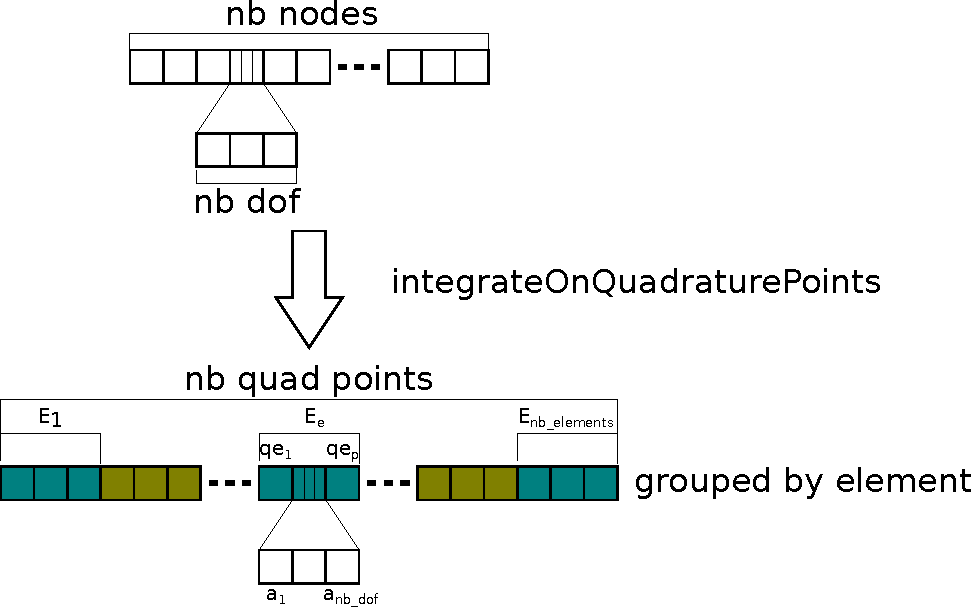
\includegraphics[width=\textwidth]{figures/interpolate}
%   \caption{Input and output  vector of interpolateOnQuadraturePoints. The output
%     Vector has nb\_quadrature\_points tuples,  the quadrature points are grouped
%     by elements (p is the number of quadrature points per element).}
%   \label{fig:interpolate-storage}
% \end{figure}

\chapter{Planning}

\begin{description}
\item[03/12/12] Cyprien: Explicit time integration scheme
\item[03/29/12] Aur\'elia: Boundary conditions
\item[04/13/12] L\'eonardo: Existing constitutive laws
\item[04/20/12] Mohadeseh: Adding a constitutive law
\item[04/27/12] Peter: Adding an element
\item[05/04/12] Till: Structural mechanics model
\item[05/11/12] Guillaume: Heat transfer model
\item[05/18/12] Marco: Cohesive elements
\item[05/25/12] Alejandro: Contact detection
\item[06/01/12] David: Contact resolution
\end{description}

\begin{figure}[!htb]
  \centering
  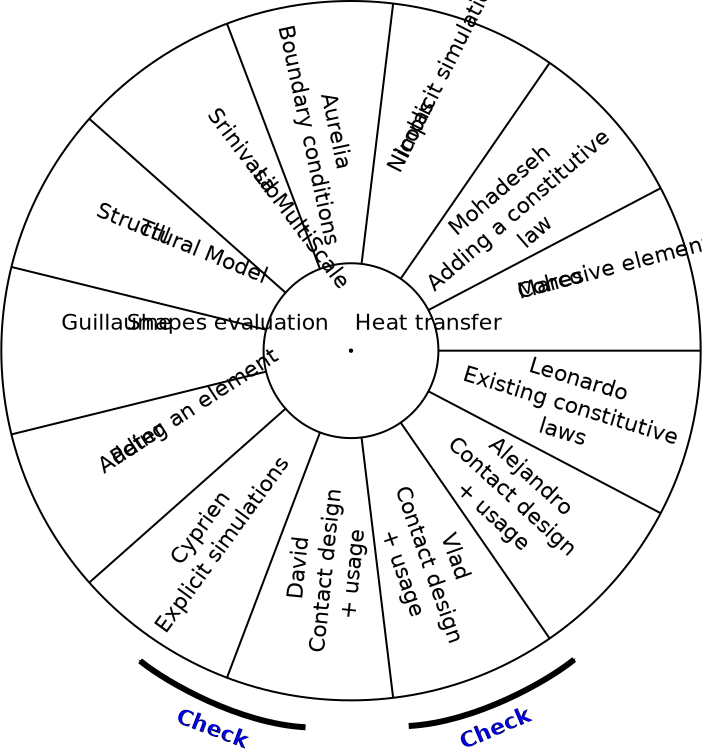
\includegraphics[width=\linewidth]{figures/doc_wheel}
  \caption{Documentation wheel\label{fig:doc_wheel}}
\end{figure}


\chapter{How to use \akantu}
\section{Getting started}
\subsection{Downloading the code}
SVN URL to get \akantu :
\begin{command}
> svn co svn+ssh://username@intranet-lsms.epfl.ch/space/repositories/SimulPack/akantu/trunk akantu
\end{command}

\subsection{Compiling \akantu}
\begin{command}
> mkdir build
> cd build
> ccmake <path to akantu sources>
\end{command}

Set the options that you need

\begin{command}
> make
> make install
\end{command}

\section{Solid Mechanics model\index{SolidMechanicsModel}}

The  solid mechanics  model is  a  specific implementation  of the  \code{Model}
interface dedicated to handle the  equation of motion. The model is instantiated
for  a  given  mesh.  It  will  create  its  own  \code{FEM}  object to  do  the
interpolation, gradient, integration and  assembly operations. A solid mechanics
model can simply be instantiated like this:
\begin{cpp}
SolidMechanicsModel model(mesh, spatial_dimension);
\end{cpp}

This model contains \code{Vectors} that will be described in the following.
\begin{description}
\item[Boundary] contains a  boolean value for each degree  of freedom specifying
  whether it is blocked or not.  if it is blocked a Dirichlet boundary condition
  is prescribed, otherwise a Neumann boundary condition can be imposed.
\item[Displacement] contains the displacements of the degrees of freedom. It can
  be either  a computed displacement for  free degrees of freedom  or an imposed
  displacement in case of blocked ones.
\item[Velocity]  contains the  velocities of  the  degrees of  freedoms. As  the
  \textbf{Displacement}, it contain computed  or imposed velocities depending on
  the nature of the degrees of freedoms.
\item[Acceleration] contains the accelerations of the degree of freedoms. As the
  \textbf{Displacement}, it contain  computed or imposed accelerations depending
  on the nature of the degrees of freedoms.
\item[Force] contains the external forces applied on the nodes.
\item[Residual] contains the difference between external and internal forces. On
  blocked degrees of freedom, \textbf{Residual} contains the support reactions.
\end{description}

Some examples for  understanding how to use this model will  be presented in the
following.

\subsection{Model setup}
\subsubsection{Creating and loading a mesh\label{sect:common:mesh}}

\begin{cpp}
  UInt spatial_dimension = 2;

  Mesh mesh(spatial_dimension);

  MeshIOMSH mesh_io;
  mesh_io.read("square.msh", mesh);
\end{cpp}

\subsubsection{Setting   initial  conditions  \label{sect:smm:initial_condition}
  \todo{Aur\'elia}}
\subsubsection{Seting        boundary        conditions\label{sect:smm:boundary}
  \todo{Aur\'elia}}

\begin{cpp}
  const  Vector<Real> & position = mesh.getNodes();
  Vector<bool> & boundary = model.getBoundary();
  Vector<Real> & displacment = model.getDisplacement();

  for (UInt n = 0; n < nb_nodes; ++n) {
    if(position(n,0) < Math::getTolerance()) boundary(n,0) = true;
    if(position(n,1) < Math::getTolerance()) boundary(n,1) = true;

    if(std::abs(position(n,0) - bar_length) < Math::getTolerance()) {
      boundary(n,0) = true;
      displacment(n,0) = 0.1;
    }
  }
\end{cpp}

These conditions put the left and bottom side on rollers.


\subsection{Static resolving\label{sect:smm:static}}

The \code{SolidMechanicsModel} class can handle different methods of resolution,
the first  one that  will be  presented is the  static case.  In this  case, the
equation to solve is as following,
\begin{equation}\label{eqn:smm:static}
  K u = f_{ext}
\end{equation}
where $K$ is the stiffness matrix, $u$ the displacement and $f_{ext}$ the external
forces applied to the system.


To     solve    such     a    problem     the    static     solver     of    the
\code{SolidMechanicsModel}\index{SolidMechanicsModel}  object is used.   First a
model has to be instantiates and  initialized.  To create the model, a mesh that
can   be   read   from   a   file   is   needed,   as   explained   in   section
\ref{sect:common:mesh}.   Once an  instance of  a  \code{SolidMechanicsModel} is
instantiated,   the   easiest   way   to   initialize   it   is   to   use   the
initFull\index{SolidMechanicsModel!initFull} function by  giving a material file
containing the material parameters, and  by specifying the good flags. The first
flag defines if we  want to use an implicit or explicit  time scheme.  It has no
importance in  this example.  The second  flag defines if  we are  interested in
solving a  dynamic problem.  In  our case, we  should set it to  \code{false} to
select a static problem.

\begin{cpp}
  SolidMechanicsModel model(mesh);
  model.initFull("material.dat", true, false);
\end{cpp}

Once the model is created and initialized we can set the boundary conditions can
be set as explained  in section \ref{sect:smm:boundary}.  The boundary condition
will prescribe  the external forces for  the free degrees  of freedoms $f_{ext}$
and  the  displacement  for  the   others.   To  completely  define  the  system
represented in  equation (\ref{eqn:smm:static}),  we must compute  the stiffness
matrix $K$. \index{SolidMechanicsModel!assembleStiffnessMatrix}

\begin{cpp}
  model.assembleStiffnessMatrix();
\end{cpp}

In   fact,  to   find  the   equilibrium   we  modify   slightly  the   equation
(\ref{eqn:smm:static}) in order to apply a Newton-Raphson convergence algorithm.

\begin{eqnarray}\label{eq:smm:static-newton-raphson}
  K^{i+1} \delta u^{i+1} &=& r = f_{ext} - f_{int} = f_{ext} - K^{i} u^{i}\\
  u^{i+1} &=& u^{i} + \delta u^{i+1}
\end{eqnarray}

In the  Newton-Raphson iteration,  we update $K$  according to  the displacement
computed at  the previous iteration and  we loop until the  forces are balanced,
that is to say $r  = 0$. To do this, we have to evaluate  $r$ and then solve the
system.\index{SolidMechanicsModel!updateResidual}
\index{SolidMechanicsModel!solveStatic}

\begin{cpp}
  model.updateResidual();
  model.solveStatic();
\end{cpp}

In an  elastic case the solution is  directly found at the  first iteration. But
for non elastic case, we need to iterate  as long as the norm of the residual is
not zero.
\begin{cpp}
  Real norm;
  UInt count = 0;
  model.updateResidual();
  while(!model.testConvergenceResidual(1e-3, norm) && (count < 100)) {
    if (prank == 0)
      std::cout << "Iter : " << ++count
                << " - residual norm : "
                << norm << std::endl;
    model.solveStatic();
    model.updateResidual();
  };
\end{cpp}

At  the   end  of  the   resolution  the  final   solution  is  stored   in  the
\code{displacement} vector.  A  full example of how to  resolve a static problem
is  presented  in   the  code  \code{example/manuel/implicit\_static.cc}.   This
example is  composed of a 2D  plate of steel,  blocked with rollers on  left and
bottom sides as  shown in figure \ref{fig:smm:static}. The  nodes from the right
side of the sample are displaced from $0.01\%$ of the length.

\begin{figure}[!htb]
  \centering
  \includegraphics{figures/implicit_static}
  \caption{Numerical setup\label{fig:smm:static}}
\end{figure}


\subsection{Dynamic methods} \label{sect:smm:Dynamic_methods}

Different ways  to solve  the equation  of motion are  implemented in  the solid
mechanics model.  The complete equations that should be solved is
\begin{equation}\label{eqn:equation-motion}
M\ddot{u} + C\dot{u} + Ku = f_{ext} -f_{int} = r
\end{equation}
where  $M$,  $C$   and  $K$  are  the  mass,   damping  and  stiffness  matrices
respectively.

In the previous section, we already  explained how to solve this equation in the
static case where $\ddot{u}  = \dot{u} = 0$.  Here we will  explain how to solve
this equation in the general case.  To reach this purpose, a time discretization
should be added. The most common discretization method in solid mechanics is the
Newmark-$\beta$ method, which is the default one in \akantu.

For the  Newmark-$\beta$ method, equation  (\ref{eqn:equation-motion}) becomes a
system  of three  equations  (see \cite{curnier92a}  \cite{hughes-83a} for  more
detail):
\begin{eqnarray}
  M     \ddot{u}_{n+1}    +     C    \dot{u}_{n+1}     +    K     u_{n+1}    &=&
  r_{n+1} \label{eqn:equation-motion-discret} \\
  u_{n+1}  &=& u_{n}  + (1  - \alpha)  \Delta t  \dot{u}_{n} +  \alpha  \Delta t
  \dot{u}_{n+1}       +       (1/2        -       \alpha)       \Delta       t^2
  \ddot{u}_n \label{eqn:finite-difference-1}\\
  \dot{u}_{n+1}  &=& \dot{u}_{n} +  (1 -  \beta) \Delta  t \ddot{u}_{n}  + \beta
  \Delta t \ddot{u}_{n+1}\label{eqn:finite-difference-2}
\end{eqnarray}

In   this  new   equations,  $\ddot{u}_n$,   $\dot{u}_n$  and   $u_n$   are  the
approximations  of  $\ddot{u}(t_n)$,   $\dot{u}(t_n)$  and  $u(t_n)$.   Equation
(\ref{eqn:equation-motion-discret})  is  the  equation  of motion  in  terms  of
approximate  solution  and  the  equations  (\ref{eqn:finite-difference-1})  and
(\ref{eqn:finite-difference-2})  are the  finite difference  formulas describing
the evolution of the approximate solutions.  The $\alpha$ and $\beta$ parameters
determine the stability and the  accuracy of the algorithm. Classical values for
$\alpha$ and $\beta$ are usually $\beta = 1/2$ for no numerical damping and $0 <
\alpha < 1/2$.

\begin{center}
  \begin{tabular}{c|l}
    $\alpha$ & Methode ($\beta = 1/2$)\\
    \hline
    $0$ & central difference\\
    $1/6$ & Fox-Goodwin (royal road)\\
    $1/3$ & Linear acceleration\\
    $1/2$ & Average acceleration (trapezoidal rule)
  \end{tabular}
\end{center}

To    be    able   to    solve    this    system    of   equations,    equations
(\ref{eqn:equation-motion-discret})-(\ref{eqn:finite-difference-2})   should  be
split in a predictor-corrector system of  equations.  Moreover, in the case of a
non-linear equation as  for the static case, an iterative  algorithm such as the
Newton-Raphson method  is applied.  Respecting  these conditions, the  system of
equation can be written as:

\noindent\textit{Predictor:}
\begin{eqnarray}
  u^{0}_{n+1} &=& u_{n}  + \Delta t \dot{u}_n +  \frac{\Delta t^2}{2} \ddot{u}_n
  \\
  \dot{u}^{0}_{n+1}  &=& \dot{u}_{n} +  \Delta t \ddot{u}_{n} \\
  \ddot{u}^{0}_{n+1} &=& \ddot{u}_{n}
\end{eqnarray}

\noindent\textit{Solve:}
\begin{eqnarray}
 (c M + d C + e K^i_{n+1}) w = f_{ext~n+1} - f^i_{int~n+1} - C \dot{u}^i_{n+1} -
 M \ddot{u}^i_{n+1}
\end{eqnarray}

\noindent\textit{Corrector:}
\begin{eqnarray}
  \ddot{u}^{i+1}_{n+1} &=& \ddot{u}^{i}_{n+1} + c w \\
  \dot{u}^{i+1}_{n+1} &=& \dot{u}^{i}_{n+1} + d w \\
  u^{i+1}_{n+1} &=& u^{i}_{n+1} + e w
\end{eqnarray}

where  $i$ is  the Newton-Raphson  iteration counter  and $c$,  $d$ and  $e$ are
parameters depending on the method used to solve the equations

\begin{center}
  \begin{tabular}{l|c|c|c|c}
    & $w$ & $e$ & $d$ & $c$\\
    \hline
    in  acceleration &$  \delta \ddot{u}$  & $\alpha  \beta \Delta  t^2$ &$\beta
    \Delta t$ &$1$\\
    in velocity &  $ \delta \dot{u}$& $1/\beta \Delta t$ &  $1$ & $\alpha \Delta
    t$\\
    in displacement &$\delta  u$ & $ 1$ & $1/\alpha \Delta  t$ & $1/\alpha \beta
    \Delta t^2$
  \end{tabular}
\end{center}

\note{If you want to use the implicit solver \akantu should be compiled at
  least with one sparse matrix solver such as Mumps\cite{mumps}.}


\subsubsection{Implicit time integration}
The example  presented here is  \code{example/manuel/implicit\_dynamic.cc}. This
example consists of a  beam blocked on one side and is on  a roller on the other
side.   A  constant  force is  applied  in  the  middle  of this  beam.   Figure
\ref{fig:smm:implicit:dynamic} presents the geometry  of this case. The material
used is a linear elastic one.

The  equation (\ref{eqn:smm:implicit})  gives  an approximation  of the  dynamic
response of the middle point of the beam.

\begin{equation}\label{eqn:smm:implicit}
  u(\frac{L}{2}, t) = \frac{1}{\pi^4} (1 - cos(\pi^2 t) +
  \frac{1}{81}(1 - cos(3^2 \pi^2 t)) +
  \frac{1}{625}(1 - cos(5^2 \pi^2 t)))
\end{equation}


\begin{figure}[!htb]
  \centering
  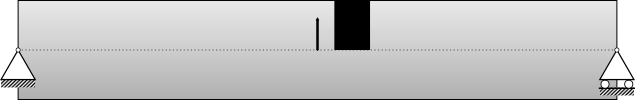
\includegraphics[scale=.6]{figures/implicit_dynamic}
  \caption{Numerical setup}
  \label{fig:smm:implicit:dynamic}
\end{figure}

To  solve  this  problem with  an  implicit  time  integration scheme,  first  a
\code{SolidMechanicsModel} object  should be created and  initialized.  Then the
initial and  boundary conditions have to  be set.  Everything is  similar to the
example in  static (section \ref{sect:smm:static}), however in  this case during
the initialization of the model, the implicit dynamic case should be selected by
setting the two flags to \code{true}.

\begin{cpp}[escapechar=\%]
  SolidMechanicsModel model(mesh);
  model.initFull("material.dat", true, true);
  /* Boundary conditions see section %\ref{sect:smm:boundary}% */
\end{cpp}

Then,   the  stiffness  matrix   $K$  and   the  mass   matrix  $M$   should  be
assembled.  Since the material is elastic in this case $C$ is equal to zero.
\index{SolidMechanicsModel!assembleStiffnessMatrix}
\index{SolidMechanicsModel!assembleMass}
\begin{cpp}
 model.assembleStiffnessMatrix();
 model.assembleMass();
\end{cpp}

Since  a dynamic  simulation is  conducted, a  time step  $\Delta t$  has  to be
specified. In the  case of implicit simulations, \akantu  use a trapezoidal rule
by  default.  That  is to  say  $\alpha  =  1/2$  and  $\beta =  1/2$  which  is
unconditionally  stable. Therefore  the value  of the  time step  can  be chosen
arbitrary.  \index{SolidMechanicsModel!setTimeStep}
\begin{cpp}
  model.setTimeStep(time_step);
\end{cpp}

Now everything is set to do the time stepping. The time loop should contains the
predictor,  the  solving  and   the  corrector  steps  with  the  Newton-Raphson
convergence algorithm even  if the material is linear.  By default the equations
are  solved  \emph{in  displacement}.   \index{SolidMechanicsModel!implicitPred}
\index{SolidMechanicsModel!implicitCorr}
\index{SolidMechanicsModel!updateResidual}
\index{SolidMechanicsModel!solveDynamic}
\begin{cpp}
  for (Real time = 0; time < simulation_time; time += time_step) {
   model.implicitPred();

   UInt count = 0;
   /// Newton-Raphson convergence loop
   do {
     model.updateResidual();
     model.solveDynamic();

     model.implicitCorr();
     ++count;
   } while(!model.testConvergenceIncrement(1e-12, error) && count < 100);

   pos << time
       << "," << displacment(node_to_print, 1)
       << "," << analytical_solution(time) << std::endl;
 }
\end{cpp}

\note{In case  of an elastic material  $K$ is constant, but  for other materials
  $K$ has to be re-assembled at each iteration.}

\note{For the convergence loop  it is a good usage to put  also a limit in terms
  of the  number of iterations  to avoid  an infinite loop  in case of  an error
  criterion too hard to reach.}

\subsubsection{Explicit dynamic}

The explicit dynamic integration scheme is based on the Newmark-$\beta$ time integration 
scheme with $\alpha=0$ (see equations \ref{eqn:equation-motion-discret}-\ref{eqn:finite-difference-2}).
In \akantu, $\beta$ is defined as $\beta=1/2$, see section \ref{sect:smm:Dynamic_methods}.

The initialization of the simulation is similar to the static and implicit dynamic version. 
The model is created from the \code{SolidMechanicsModel} class. 
In the initialization, the use of the explicit scheme is defined by setting both flags 
to false (see section \ref{sect:smm:static}). 

\begin{cpp}
  SolidMechanicsModel model(mesh);
  model.initFull("material.dat", false, false);
\end{cpp}
\index{SolidMechanicsModel!initFull}

\note{Writting \code{model.initFull("material.dat");} is equivalent to setting both flags to false, as this is the default case.}

The implemented explicit scheme in \akantu uses a lumped mass matrix $M$ (which reduces the computation cost). This matrix is assembled by distributing the mass of each element onto its nodes. The resulting $M$ is therefore a diagonal matrix.

\begin{cpp}
  model.assembleMassLumped();
\end{cpp}
\index{SolidMechanicsModel!assembleMassLumped}

The explicit integration scheme is conditionally stable. The time step has to be smaller than the stable time step which is obtained in \akantu as following: 

\begin{cpp}
  time_step = model.getStableTimeStep();
\end{cpp}
\index{SolidMechanicsModel!StableTimeStep}

The stable time step is defined as

\begin{equation}
  \Delta t = \Delta x \sqrt{\frac{\rho}{2 \mu +\lambda}}
\end{equation}
\label{eqn:smm:explicit:stabletime}

where $\Delta x$ is characteristic length, $\mu$ and $\lambda$ are the 
first and second Lame's coefficients and $\rho$ the density. The stable time step corresponds to the time the fastest wave (the compressive wave) needs, to travel the characteristic length of the mesh. 
However, note that if the time step of the computation is equal to the stable time step, 
the simulation remains unstable. Therefore, is it necessary to impose a time step that is smaller than the stable time step. One can, for instance, multiply  the stable time step by a time factor smaller than one. 

\begin{cpp}
  const Real time_factor = 0.1;
  Real applied_time_step = time_step * time_factor;
  model.setTimeStep(applied_time_step);
\end{cpp}
\index{SolidMechanicsModel!setTimeStep}
 
The initial displacement and velocity fields are, by default, equal to zero if not given specifically by the user (see \ref{sect:smm:initial_condition}).

The loop allows, for each time step, to update the displacement, velocity 
and acceleration fields which are given by the Newmark$-\beta$ equations with $\beta=1/2$ 
and $\alpha=0$.

\begin{cpp}
  for (UInt s = 1; (s-1)*applied_time_step < total_time; ++s) {
    model.explicitPred();
    model.updateResidual();
    model.updateAcceleration();
    model.explicitCorr();
  }
\end{cpp}
\index{SolidMechanicsModel!explicitPred}
\index{SolidMechanicsModel!explicitCorr}
\index{SolidMechanicsModel!updateResidual}
\index{SolidMechanicsModel!updateAcceleration}

In the code shown above, the explicit loop contains four steps:
\begin{itemize}
\item \code{model.explicitPred()} allows to compute the displacement field at $t+1$ and a 
part of the velocity field at $t+1$, denoted by $\dot{u}_{n+1/2}$, which will be used later in 
the \code{model.explicitCorr()}. The solved equations are :

\begin{eqnarray}
  u_{n+1}        &=& u_{n} +  \Delta t \dot{u}_{n} + \frac{\Delta t^2}{2} \ddot{u}_{n} \\
  \dot{u}_{n+1/2}  &=& \dot{u}_{n} +  \Delta t  \ddot{u}_{n}
  \label{eqn:smm:explicit:onehalfvelocity}
\end{eqnarray}

\item \code{model.updateResidual()} and \code{model.updateAcceleration()} allow to 
solve the equation which gives the acceleration increment $\delta \ddot{u}$:

\begin{eqnarray}
 (M + \frac{1}{2} \Delta t C + ) \delta \ddot{u} = f_{ext} - f_{int~n+1} - C \dot{u}_{n} - M \ddot{u}_{n}
\end{eqnarray}

\note{The internal force $f_{int~n+1}$ is computed from the displacement $u_{n+1}$ based on the constitutive law.} 

\item \code{model.explicitCorr()} computes the velocity and acceleration fields at $t+1$:

\begin{eqnarray}
\dot{u}_{n+1}  &=& \dot{u}_{n+1/2} + \frac{\Delta t}{2} \delta \ddot{u} \\
\ddot{u}_{n+1}  &=& \ddot{u}_{n} +  \delta \ddot{u}
\end{eqnarray}

\end{itemize}
The use of the explicit integration scheme is illustrated on an exemple
(see \code{example/manuel/explicit\_dynamic.cc}).
This example models the propagation of a wave in a steel beam. The beam 
is blocked on one side and a displacement is applied on the other side, as shown in figure \ref{fig:smm:explicit}. 

\begin{figure}[!htb]
  \centering
  \includegraphics[scale=.6]{figures/explicit_dynamic}
  \caption{Numerical setup \label{fig:smm:explicit}}
\end{figure}

The length and height of the beam are $10$m and $1$m, respectively. The material is 
linear elastic, homogeneous and isotropic (density: $7800$kg.m$^{-3}$, Young's 
modulus: $210.10^{9}$Pa and Poisson's ratio: $0.3$). The imposed displacement is equal 
to $\Delta u = 0.05$m. The potential, kinetic and total energies are computed. 
The time factor is equal to $0.1$. The total simulated time is $0.01s$.

\subsection{Constitutive laws\todo{L\'eonardo}}
\subsubsection{Elastic}
\subsubsection{Caughey}
\subsubsection{Neo-hookean}
\subsubsection{Visco-elastic}
\subsubsection{Damage Marigo}
\subsubsection{Damage Mazars}

\subsection{Adding a new constitutive law\todo{Mohadeseh}}

\subsection{Contact\todo{Alejendro, David, Vlad}}

\subsection{Cohesive laws\todo{Marco}}


\section{Structural Mechanics model\todo{Till}}

\section{Heat Transfer model\todo{Guillaume}}

% \subsection{Contact Neighbor Structure}

% The contact neighbor  structure is an interface which is  ment to be heritated
% from in order  to implement different type of  contact neighbor structures. It
% has the following protected attributes:
% \begin{itemize}
%   \item id
%   \item contact search
%   \item master surface
%   \item neighbor list
%   \item type
% \end{itemize}
% The \emph{id} and the \emph{type}  are characteristics of the contact neighcor
% structure object which  define its id and its  type. The \emph{contact search}
% attribute  is  the associated  contact  search  object  to the  given  contact
% neighbor structure  object. The \emph{master  surface} attribute is the  id of
% the  associated master  surface for  which the  neighbor structure  has  to be
% built. Finally, the neighbor list  is the constructed neighbor structure which
% defines the  impactor nodes  that are  in the neighborhood  of either  a given
% master  node or  a given  master  surface element,  depending on  the type  of
% contact neighbor structure.

% The contact neighbor structure provides the accessor \emph{getNeighborList} to
% the constructed  neighbor list and forces  the heritated classes  to provide a
% public \emph{initNeighborStructure}  function, which initializes  the neighbor
% structure,  as well  as a  public  \emph{update} function,  which updates  the
% neighbor structure.

% \subsubsection{Regular Grid Neighbor Structure}

% The regular  grid neighbor structure builds  a regular grid  around the master
% surface and  uses it in  order to construct  the neighbor list.  This neighbor
% structure can construct both types of neighbor list, the


% \subsection{Implementation of a new solid mechanics problem}

% Let us imagine you want to implement a new material called
% "toto" in akantu. The have to complete the following steps (in
% any order) :
% \begin{enumerate}
% \item
% Declare a new material in the file
%      \textit{Akantu/model/solid\_mechanics/solid\_mechanics\_model\_material.cc}.
% You have to had this line after the list of possible cases
% \begin{verbatim}else if(mat\_type == "toto") material =
%      parser.readMaterialObject<MaterialToto>(*this,mat_id);
% \end{verbatim}


% \item
% Include the new material in \textit{Akantu/model/solid\_mechanics/material.hh} \\
% add the line :
% \begin{verbatim}
% #include "materials/material\_toto.hh"
% \end{verbatim}

% \item
% For compilation include the new file to compile in
%      \textit{Akantu/CMakelist.txt} by adding
% \begin{verbatim}
% model/solid_mechanics/materials/material_toto.cc
% \end{verbatim}
% \item
% In \textit{Akantu/model/solid\_mechanics/materials}, create (or copy from
%      an allready existing material) the three following files :\\
% - material\_toto.cc\\
% - material\_toto.hh\\
% - material\_toto\_inline\_impl.cc

% \item
% Modify the files !

% \end{enumerate}
\printindex

\bibliography{biblio}

\end{document}
